% ****** Start of file apssamp.tex ******
%
%   This file is part of the APS files in the REVTeX 4.2 distribution.
%   Version 4.2a of REVTeX, December 2014
%
%   Copyright (c) 2014 The American Physical Society.
%
%   See the REVTeX 4 README file for restrictions and more information.
%
% TeX'ing this file requires that you have AMS-LaTeX 2.0 installed
% as well as the rest of the prerequisites for REVTeX 4.2
%
% See the REVTeX 4 README file
% It also requires running BibTeX. The commands are as follows:
%
%  1)  latex apssamp.tex
%  2)  bibtex apssamp
%  3)  latex apssamp.tex
%  4)  latex apssamp.tex
%
\documentclass[%
 reprint,
%superscriptaddress,
%groupedaddress,
%unsortedaddress,
%runinaddress,
%frontmatterverbose, 
%preprint,
%preprintnumbers,
%nofootinbib,
%nobibnotes,
%bibnotes,
 amsmath,amssymb,
 aps,
%pra,
%prb,
%rmp,
%prstab,
%prstper,
%floatfix,
]{revtex4-2}

\usepackage{graphicx}% Include figure files
\usepackage{dcolumn}% Align table columns on decimal point
\usepackage{bm}% bold math
%\usepackage{hyperref}% add hypertext capabilities
%\usepackage[mathlines]{lineno}% Enable numbering of text and display math
%\linenumbers\relax % Commence numbering lines

%\usepackage[showframe,%Uncomment any one of the following lines to test 
%%scale=0.7, marginratio={1:1, 2:3}, ignoreall,% default settings
%%text={7in,10in},centering,
%%margin=1.5in,
%%total={6.5in,8.75in}, top=1.2in, left=0.9in, includefoot,
%%height=10in,a5paper,hmargin={3cm,0.8in},
%]{geometry}

\graphicspath{ 
{./images}
}

\usepackage{ mathrsfs }
\newcommand{\bb}[1]
{\mathbb{#1}}
\newcommand{\gap}
{\vspace{5mm}}
\newcommand{\cpp}[2]
{{\centering
\includegraphics[scale=#2]{#1}
\par}}

\begin{document}

\preprint{APS/123-QED}

\title{Hybrid evolutionary algorithm and gradient-based algorithm for multi-objective optimization}% Force line breaks with \\

\author{%
Zhang Kenneth
}
\author{Wang Gui Zheng}%
\author{Xu Kuang Jie}
\affiliation{%
Southern University of Science and Technology }%


\begin{abstract}
Traditional multi-objective optimization problems (MOP) have been rigorously studied and various algorithms based on the principles of evolution, such as NSGA-II, SPEA-II, MOEA/D, and SMS-EMOA, have been proposed. An alternative approach to solving the MOP includes the calculation of gradients and guiding the search towards some local optimum. In this paper, we present a hybrid algorithm combining the effects of gradient-descent algorithms as well as evolutionary algorithms.
\end{abstract}

%\keywords{Suggested keywords}%Use showkeys class option if keyword
                              %display desired
\maketitle

%\tableofcontents

\section{\label{sec:level1}	
An overview of the MOP
\protect\\
and its related concepts}

A multiobjective optimization problem (MOP) can be stated as follows: \cite{MOEA-D}
\begin{eqnarray}
\text{minimize } F(\bold{x}) &&= (f_1(\bold{x}), \dots, f_m(\bold{x}))^T \nonumber\\
\text{subject to } \bold{x}\  &&\in \Omega
\end{eqnarray}

where $\Omega$ is the \textit{decision (variable) space, } $F : \Omega \to \bb{R}^m$ consists of $m$ real-valued objective functions and $\bb{R}^m$ is called the objective space. The \textit{attainable objective set} is defined as the set $\{F(\bold{x}) \ |\  \bold{x} \in \Omega\}$.

Assuming minimization of the objective functions, among solution vectors $\bold{y}, \bold{y}' \in \bb{R}^m$, a partial order is defined by the \textit{dominance relation} ``$\prec$'': \cite{SMS-EMOA}
\begin{eqnarray}
\bold{y} \prec \bold{y}' (\bold{y} \text{ dominates } \bold{y}') \nonumber\\
\iff
\forall i \in \{1, \dots, m\}: y_i \leq y_i' \nonumber\\
\text{and } \exists j \in \{1, \dots, m\} : y_j < y_j'
\end{eqnarray}

For $\bold{x}, \bold{x}' \in \Omega$, we write $\bold{x} \prec \bold{x}' \iff F(x) \prec f(x')$. The minimal elements of the dominated relation are called \textit{Pareto-optimal} and the set of Pareto-optimal decision vectors is called \textit{Pareto(-optimal) set}: 
\begin{equation}
\{x \in \Omega\ | \ \nexists \bold{x}' \in \Omega: \bold{x}' \prec \bold{x}\}
\end{equation}

The corresponding image under $F$ in the solution space $\bb{R}^m$ is called \textit{Pareto front}. A point in the search space is called \textit{non-dominated} within a set $A \subset \Omega$ if there is no point in $A$ dominating it.


\begin{figure}[b]
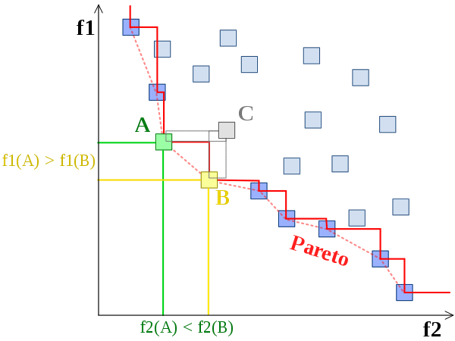
\includegraphics[width=0.25\textwidth]{fig_0}% Here is how to import EPS art
\caption{\label{fig:pareto-optimality} Concept of pareto-optimality. Blue squares are the non-dominated solutions, white squares are dominated solutions.}
\end{figure}


\subsection{\label{sec:level2}Elitism}

\cite{AunifiedmodelLaumanns}
Elitism has always been a major topic of discussion in the evolutionary computation community. This mainly concerns
cross-generational interaction. Though it is clear that all natural
individuals have a limited lifespan, there is no general
answer to how this concept should be applied to evolutionary
algorithms. Interpretations are diverse: Canonical genetic algorithms,
for instance, allow no parental survivability at all.
In generation gap methods at least a fraction of the next generation
is reserved for good parents, and in the $(\mu + \lambda)$ evolution strategies parents live as long as they are surpassed by better offspring.

The question of when to accept a newly generated solution,
in spite of previously found ones, arises in all kinds
of iterative melioration processes, e.g. simulated annealing,
where the probability of accepting (temporary) worsening is
controlled by a `cooling' schedule.

As opposed to single-objective optimization, the question of
elitism becomes even more complicated with MOEAs. Here,
the set of decision alternatives is no longer totally ordered,
and alternatives might be incomparable. This makes an `elitist'
decision difficult, so a number of different MOEA implementations
emerge with elitistic features. These features may
be classified along different criteria:

\begin{itemize}
\item
Using a secondary `elitist' population vs. implicit elitism through a `plus' selection as in evolution strategies;
\item
The elitism strategy, or how the elitist population is updated;
\item
The evaluation strategy, or how the elite individuals affect the fitness assignment of the current generation and vice versa;
\item
The re-insertion strategy, or how elite individuals take part in the production of offspring;
\item
The control flow, or when archiving and re-insertion take place.
\end{itemize}

As this classification is not hierarchical, algorithms can arbitrarily
combine different features.

\subsection{\label{sec:level2}Hypervolume}

\cite{SMS-EMOA}A variety of quality indicators is used in order to measure the quality of Pareto front approximations. Among them, the \textit{hypervolume measure} or $\mathscr{S}$ \textit{metric} is of outstanding importance. It is a quality indicator that
rewards the convergence towards the Pareto front as well as the representative distribution of points along the
front. The hypervolume measure was originally proposed by Zitzler and Thiele, who called it the \textit{size of dominated space}. Let $\Lambda$ denote the Lebesgue measure, then the $\mathscr{S}$ metric is defined as:
\begin{equation}
\mathscr{S}(B, \bold{y}_\text{ref}) := \Lambda \bigg(
\bigcup_{\bold{y} \in B} \{\bold{y}' \ | \ \bold{y} \prec \bold{y}' \prec \bold{y}_\text{ref} \} \bigg),
B \subset \bb{R}^m
\end{equation}

Here, $\bold{y}_\text{ref} \in \bb{R}^m$ denotes a reference point that should be dominated by all Pareto-optimal solutions.

Fleischer [5] proved that, given a finite search space and a reference point, maximisation of the hypervolume
measure is equivalent to finding the Pareto set. Therefore, a set of bounded size which obtains the
maximal S metric value that is possible for the given size, only consists of Pareto-optimal solutions. It has
been empirically observed that for a fixed number of points, the maximisation of the hypervolume metric
yields subsets of the Pareto front which are well-distributed (cf. [6,7]). \cite{SMS-EMOA}

\begin{figure}
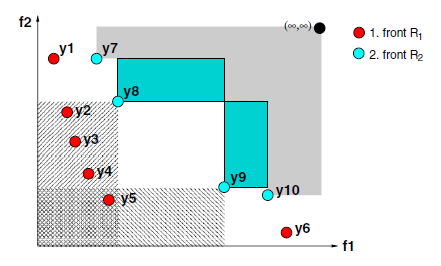
\includegraphics[width=0.5\textwidth]{fig_2}
\caption{\label{fig:hypervolume} Concept of hypervolume. Red circles are non-dominated front whereas blue circles are the next front. The hypervolume for the second front is indicated as the union of the gray shade and the blue shade.}
\end{figure}



\section{\label{sec:level1}	
A discussion of \protect\\
contemporary MOEAs}

Multi-Objective Evolutionary Algorithms (MOEAs) have emerged as a powerful and broadly applicable subset of evolutionary computation techniques that effectively address multi-objective optimization problems (MOPs). MOPs are characterized by the need to optimize more than one conflicting objective, necessitating a search for a set of optimal solutions, known as Pareto optimal solutions. The advent of Vector Evaluated Genetic Algorithm (VEGA) by Schaffer et al. in 1985 pioneered the generalization of Genetic Algorithms (GAs) to handle vector-valued (multi-objective) fitness functions. However, it was constrained to a single feature optimization, prompting a surge in the development of more sophisticated approaches.

\begin{figure}[b]
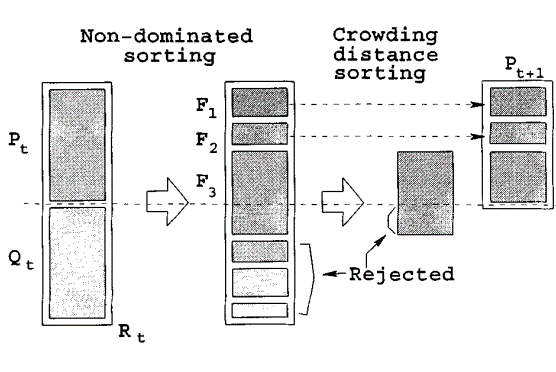
\includegraphics[width=0.5\textwidth]{fig_1}
\caption{\label{fig:NSGA-II} NSGA-II utilizes an external archive (elitism) to guide the selection process of the next group of population.}
\end{figure}

\begin{figure*}
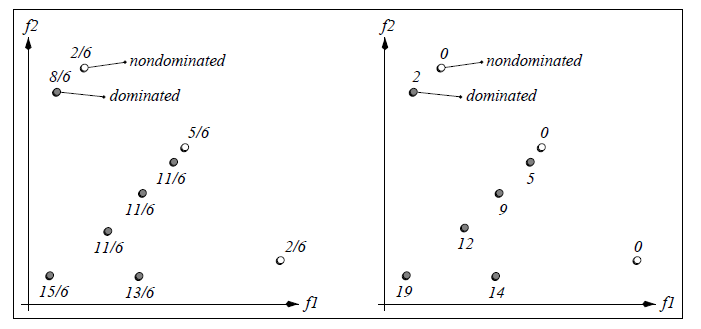
\includegraphics[width=0.8\textwidth]{fig_3}
\caption{\label{fig:SPEA-II} SPEA-II using a fitness assignment scheme based on the concept of Pareto strength.}
\end{figure*}

Building upon the foundational work of VEGA, Horn et al.'s Niched Pareto Genetic Algorithm (NPGA) in 1994 introduced the concept of niching and the sharing parameter, which allows the algorithm to maintain a diverse population of solutions. The addition of a comparison set was particularly novel, allowing the algorithm to filter out inferior solutions efficiently.

Further refinement came with Fonseca \& Fleming's Multiple Objective Genetic Algorithms (MOGA) in 1993, which pioneered the use of domination-based ranking for fitness assignment. MOGA also discussed niche formation using both phenotypic and genotypic distances, highlighting the importance of genetic encoding in representing phenotype similarities.

The integration of random weight in Murata \& Ishibuchi's 1995 study introduced an essential aspect of diversity maintenance, allowing for broader exploration of the solution space. This concept was enhanced by Ishibuchi et al. in 1998 with Multi-Objective Genetic Local Search (MOGLS), which combined random weight vectors with local search techniques.

Deb et al.'s NSGA-I in 1994 and its successor, NSGA-II in 2002, marked significant improvements in computational efficiency and solution quality. NSGA-II's introduction of elitism, non-dominated sorting, and crowding distances provided an elegant method of maintaining diversity while being computationally tractable, a considerable advancement from its predecessors.

The Pareto Archive Evolution Strategy (PAES) by Knowles et al. in 1999 and the Pareto Envelope-based Selection Algorithm (PESA) by Corne et al. in 2000, took the evolution strategies route, focusing on archiving and hypergrid techniques to preserve solution quality across generations.

Zitzler et al.'s Strength Pareto Evolutionary Algorithm (SPEA) in 1999 and SPEA-II in 2001 provided a holistic approach that assimilated characteristics of VEGA, MOGA, NPGA, and NSGA. The introduction of fine-grained strength fitness assignment and nearest neighbor density estimation in SPEA-II represented a significant step towards the maintenance of boundary solutions and the enhancement of solution quality.

In 2007, Zhang et al. introduced Multi-Objective Evolutionary Algorithm based on Decomposition (MOEA/D), which represented a paradigm shift in handling MOPs. By decomposing a multi-objective problem into several single-objective subproblems and optimizing them simultaneously, MOEA/D provided an effective means of exploring and exploiting the problem space.

Somewhat recently, SMS-EMOA by Beume et al. in 2006 presented an approach centered around the hypervolume measure, offering a fitness metric that quantified the “size of the dominated space.” This metric provided an intuitively appealing and direct method of assessing solution quality in terms of the volume of the objective space that is dominated by the Pareto front. This performance indicator shall be the foundation of our proposed work.

\section{\label{sec:level1}	
A short review of Gradient-based Multi-objective Algorithms}


The Multiple-Gradient-Descent Algorithm (MGDA) is an innovative approach in multi-objective optimization that capitalizes on the concept of considering multiple gradients simultaneously. Unlike traditional gradient descent, which is tailored for single-objective problems, MGDA identifies a search direction that is descent for all objectives. This is accomplished through the computation of a common descent direction derived from the gradients of all objectives, seeking a compromise between them. The algorithm is particularly adept at navigating the trade-off surface defined by conflicting objectives, steering the solution towards Pareto optimality.

Pareto-Set Learning (PSL) represents a more nuanced approach to multi-objective optimization. It extends beyond the mere pursuit of Pareto front by learning the underlying structure of the Pareto set. PSL employs a collaborative filtering method that harnesses the gradients of the objectives to learn a model of the Pareto set. This model is then utilized to predict Pareto-optimal solutions. PSL’s strength lies in its ability to incorporate the geometry of the problem, which often results in a more efficient convergence to high-quality Pareto-optimal solutions compared to algorithms that do not leverage such information.

To our great interest is the usage of the hypervolume indicator in the SMS-EMOA algorithm. A recent algorithm called Hypervolume Indicator Gradient Ascent
Multi-objective Optimization (HIGA-MO) combined the idea of gradient descent with the hypervolume indicator. HIGA-MO introduces a novel perspective by focusing on the hypervolume indicator, a set performance measure that reflects the size of the space dominated by the Pareto front. By ascending the gradient of the hypervolume indicator, HIGA-MO seeks to expand the dominated space, effectively pushing the Pareto front towards better trade-offs. This approach is particularly powerful as the hypervolume indicator inherently balances the spread and convergence of the solutions. HIGA-MO is adept at uncovering a set of non-dominated solutions that provides a comprehensive portrayal of the trade-offs involved in multi-objective scenarios.

\section{\label{sec:level1}	
Background concepts in conducting gradient algorithms}

To utilize gradient information, we assume that each objective function $f_i$ is continuous differentiable \textit{almost everywhere} in $S_i$. Thus, the MOP can be formulated as follows: \cite{HIGA-MO}
\begin{equation}
\max_{\bold{x}\in S}F(x), \ \Omega = \bigcap_{i=1}^m \Omega_i \subseteq \bb{R}^d
\end{equation}

where $F(x) = [f_1(\bold{x}), \dots, f_m(\bold{x})]^T$ is a vector-valued function composed of $m$ objective functions. This aligns with our earlier definition of the MOP. Due to the continuous differentiability assumption on each objective function, $F$ is
again continuous differentiable almost everywhere in S. The gradient information
is expressed as transpose of the Jacobian matrix as follows:
\begin{equation}
\frac{\partial F(\bold{x})}{\partial \bold{x}}
=
[
\nabla f_1(\bold{x}), \dots, \nabla f_m(\bold{x})]
\end{equation}

In addition, it is assumed that each gradient vector above (column vector) can be
computed either analytically or numerically. In MOPs, a set of decision vectors
are moved in \textit{decision space} $\Omega$ to approximate the Pareto efficient set.

\section{\label{sec:level1}	
An efficient operator utilizing\protect\\ gradient information of Pareto-optimal solutions
}

\begin{figure}[b]
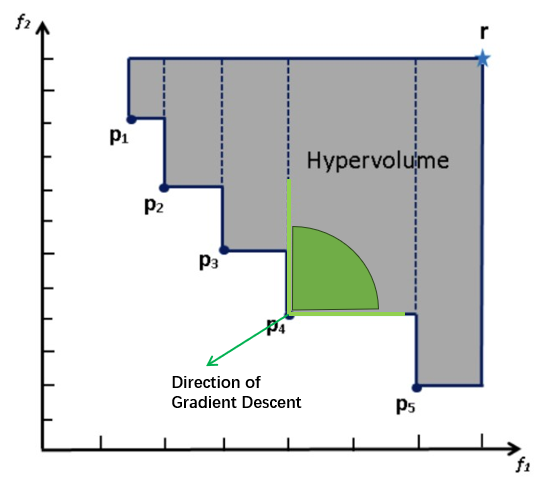
\includegraphics[width=0.3\textwidth]{fig_4}
\caption{\label{fig:Migration operator} The concept of migration operator using gradient information of a pareto-optimal solution}
\end{figure}

Usually gradient descent information is used on a single point to determine the direction of search space. We propose an efficient searching method using the `migration' operator. We define some terms and make analogies to a natural phenomena: In classical theories of anthropology and sociology, a `clan' consists of a `clan leader' and dominated `clan members'. We derive the concept of `leader' by referring to non-dominated solutions as `leading solutions', and the set of populations dominated by this `leading solutions' is named a `clan'. We introduce a `migration' operator where the `leader' determines first its local Gradient information, and establishes a search direction in which the entire `clan' will move towards; however, during the process an indicator needs to be evaluated to determine the efficiency and utility of the migration step. Here we use the HV-indicator to determine solutions that improves the overall hypervolume. An elitist approach is conducted by maintaining a Pareto Archive which the `migration step' can compare the hypervolume with, and we collectively discard individuals that degrade the level of hypervolume after the migration step.
% The \nocite command causes all entries in a bibliography to be printed out
% whether or not they are actually referenced in the text. This is appropriate
% for the sample file to show the different styles of references, but authors
% most likely will not want to use it.
\nocite{*}

\newpage

\bibliography{report_mNotes}% Produces the bibliography via BibTeX.

\end{document}
%
% ****** End of file apssamp.tex ******
